\documentclass{beamer}
\usetheme{CambridgeUS}
\DeclareGraphicsExtensions{.pdf, .jpg, .gif, .bmp}
\usepackage{amsmath,amsthm}
%\usepackage[numbers]{natbib}
\usepackage{graphicx}
\usepackage{hyperref}
%\def\newblock{} %this is needed for natbib
\newcommand{\var}{\mathrm{var}}
\newcommand{\cov}{\mathrm{cov}}
\newcommand{\E}{\mathbb{E}}
\newcommand{\N}{\mathcal{N}}
\newcommand{\law}{\overset{D}{\rightarrow}}
\newcommand{\prob}{\overset{P}{\rightarrow}}

%\newtheorem{proposition}{Proposition}
%\newtheorem{theorem}{Theorem}

\begin{document}
\title[Two-Sample Kernel Tests]{Thesis Proposal: Two-Sample Kernel Based Tests}
\author[N. Ray with S. Holmes]{Nelson Ray (joint work with Susan
  Holmes)}
\institute[Stanford]{Stanford University}
\date{\today}

\begin{frame}
  \titlepage
\end{frame}

% \begin{frame}{The paper}
%   \begin{figure}
%     \includegraphics[scale=.55]{title.png}
%   \end{figure}
% \end{frame}

\begin{frame}{Outline}
  \begin{itemize}
  \item Motivation: breast cancer study with heterogeneous data \pause
  \item Friedman's two-sample test \cite{friedman30908multivariate}:
    leverage regression and classification techniques \pause
  \item Univariate data and linear predictions: permutation t-test \pause
  \item Permutation dependence: Stein's method for rates of
    convergence \pause
  \item Simulations to inform bounds in proof (experimental
    mathematics) \pause
  \item Twitter example for text data \pause
  \item Future work: theory for general case, heterogeneous data and
    combining kernels
  \end{itemize}
\end{frame}

\begin{frame}{Breast Cancer Data: Spatial}
  \begin{figure}
    \centering
    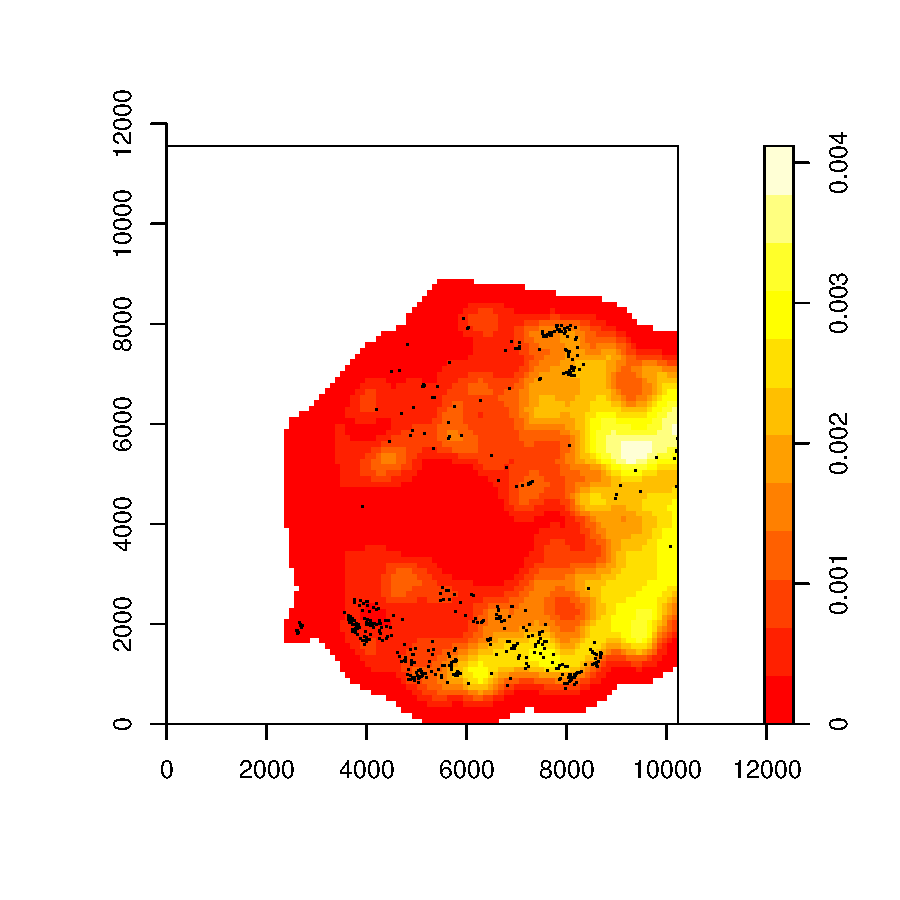
\includegraphics[scale=.5]{Fig2healthyDC.pdf}
  \end{figure}
\end{frame}

\begin{frame}{Breast Cancer Data: Survival}
  \begin{figure}
    \centering
    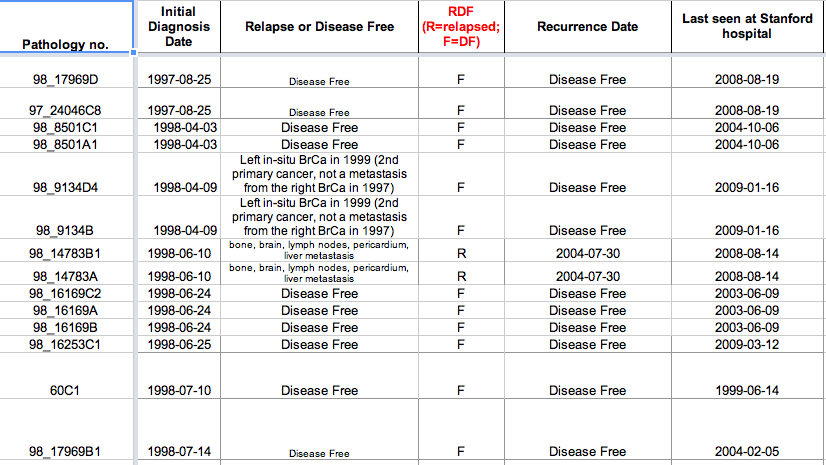
\includegraphics[scale=.5]{survival.png}
  \end{figure}
\end{frame}

\begin{frame}{Breast Cancer Data: Medical}
  \begin{figure}
    \centering
    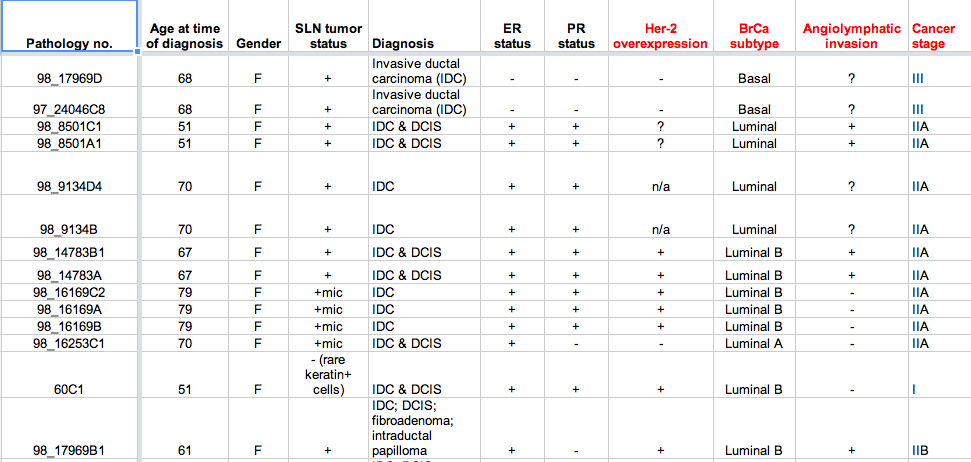
\includegraphics[scale=.5]{medical.png}
  \end{figure}
\end{frame}

\begin{frame}{Breast Cancer Study}
  \begin{itemize}
  \item How do you deal with the data integration problem? \pause
  \item Kernel methods \pause
  \item Are there any differences (spatial, medical) between women who
    relapse and those who remain disease free? \pause 
  \item Two-sample tests
  \end{itemize}
\end{frame}

\begin{frame}{Friedman's Two-Sample Test}
  $\{\mathbf{x}_i\}_1^N$ from $p(\mathbf{x})$ and
  $\{\mathbf{z}_i\}_1^M$ from $q(\mathbf{x})$ testing \\ 
  $\mathcal{H}_A$: $p \neq q$ against $\mathcal{H}_0$: $p = q$ \pause
  \begin{enumerate}
  \item Pool the two samples $\{\mathbf{u}_i\}_1^{N+M} =
    \{\mathbf{x}_i\}_1^{N} \cup \{\mathbf{z}_i\}_1^{M}$. \pause
  \item Assign label $y_i = 1$ to the first group and $y_i = -$1 to
    the second group. \pause
  \item Apply a binary classification learning machine $f$ to the training
    data to score the observations $\{s_i =
    f(\mathbf{u}_i)\}_1^{N+M}$. \pause
  \item Calculate a univariate two-sample test statistic $T =
    T(\{s_i\}_1^N,\{s_i\}_{N+1}^{N+M})$. \pause
  \item Determine the permutation null distribution of the above
    statistic to yield a p-value.
  \end{enumerate}  
\end{frame}

\begin{frame}{Permutation T-test Connection}
  With univariate data and linear predictions, Friedman's test reduces
  to the permutation t-test.  \pause
  \newline
  \newline 
  With multivariate data, the test is close to Hotelling's
  $T^2$-test. \pause
  \newline
  \newline 
  Strategy: Analyze the simple case (univariate/linear) and attempt to
  generalize. 
\end{frame}

\begin{frame}{Other Work}
  \begin{itemize}
  \item Fisher (1935) \cite{fisher1935design} proposed distribution
    free randomization test.  \pause
  \item Lehmann \cite{lehmann1999elements} proved a normal convergence
    result for the randomization distribution. \pause
  \item Bentkus et al. \cite{bentkus1996berry}, Shao
    \cite{shao2005explicit} proved Berry-Esseen bounds for
    Student's $t$-statistic in independent (but not i.d.) case. 
  \end{itemize}
\end{frame}

\begin{frame}{Stein's Method and the Randomization Distribution}
  Let $\Phi(t)$ denote the standard normal CDF and $T$ be a random
  variable that is distributed according to our permutation $t$ null
  distribution. 

  Can we get a bound on
  \begin{equation*}
    \sup_{t \in \mathbb{R}} |P(T \leq t) - \Phi(t)|?
  \end{equation*}
  \pause

  We are finishing up a proof using the method of exchangeable pairs
  where our bound is $O(N^{-1/4})$.
\end{frame}

\begin{frame}{Proof Ideas}
  Chen et al. \cite{chen2010normal}:
  \begin{theorem}
    If $T$, $T'$ are mean 0, variance 1 exchangeable random variables
    satisfying
    \begin{equation*}
      \E[T-T'|T] = \lambda(T-R)    
    \end{equation*}
    for some $\lambda \in (0,1)$ and some random variable $R$, then 
    \begin{equation*}
      \sup_{t \in \mathbb{R}} |P(T \leq t) - \Phi(t)| \leq B +
      (2\pi)^{-1/4}\sqrt{\frac{\E|T'-T|^3}{\lambda}} + \E|R|,
    \end{equation*}
    where $B \leq \frac{\Theta}{2\lambda}$ and $\Theta =
    \sqrt{\var(\E[(T'-T)^2|T])}$. 
  \end{theorem}
\end{frame}

\begin{frame}{Proof Ideas}
  \begin{itemize}
  \item  Attempts to follow Stein's \cite{stein1986approximate} 
    proof of the Hoeffding combinatorial central limit theorem \pause
  \item  General contraction property, or ``approximate case,''
    from Stein et al. \cite{stein2004use} and Holmes
    \cite{holmes2004stein} \pause
  \item Computational and simulation aided proof (Borwein
    \cite{borwein2004mathematics}) with efficient $t$-statistic
    updates similar to Diaconis et al. \cite{diaconis1994gray}
  \end{itemize}
\end{frame}

\begin{frame}{Exchangeable Pair}
  For simplicity, assume $M = N$.  We have data $\{u_1, \ldots, u_N,
  u_{N+1}, \ldots, u_{2N}\}$.  Take a uniformly random permutation
  $\pi$, and let 
  \begin{equation*}
    T = T \left (\{u_{\pi(i)}\}_{i=1}^{N},
      \{u_{\pi(i)}\}_{i=N+1}^{2N} \right).
  \end{equation*}
  \pause
  
  Let $(I, J)$ be a uniformly random transposition between groups:
  over the $N^2$ cases where $1 \leq I \leq N$ and $N + 1 \leq J \leq
  2N$. Then 
  \begin{equation*}
    T' = T \left (\{u_{\pi \circ (I, J) (i)}\}_{i=1}^{N},
      \{u_{\pi \circ (I, J) (i)}\}_{i=N+1}^{2N} \right).
  \end{equation*}

  $T$ and $T'$ form an exchangeable pair.
\end{frame}

\begin{frame}{Bound Calculations}
  \begin{align*}
    \sup_{t \in \mathbb{R}} |P(T \leq t) - \Phi(t)| &\leq 
  \underbrace{\frac{\sqrt{\var(\E[(T'-T)^2|T])}}{2\lambda}}_1 \\ &+ 
  \underbrace{(2\pi)^{-1/4}\sqrt{\frac{\E|T'-T|^3}{\lambda}}}_2 \\ &+ 
  \underbrace{\E|-\frac{1}{\lambda}\E[T-T'|T]+T|}_3
  \end{align*}
\end{frame}

\begin{frame}{Simulation Information}
  \begin{enumerate}
  \item Draw samples $\{\mathbf{x}_i\}_1^{N}$ and
    $\{\mathbf{z}_i\}_1^{N}$. \pause
  \item Pick a permutation $\pi$ uniformly at random. \pause
  \item Calculate the two-sample $t$-statistic, $T$, on the permuted
    data. \pause
  \item Calculate the $N^2$ values of $T'$ resulting from all
    allowable transpositions $(I, J)$ that swap an $x$ for a $z$.
  \item Calculate conditional expectations with respect to $T$ and
    condition on $T$ for the unconditional expectations. \pause
  \item Average over many values of $T$, and repeat for a sequence of
    $N$'s.  
  \end{enumerate}
\end{frame}

\begin{frame}[fragile]{Simulated Data}
\begin{verbatim}
                  T     Tprime    N       lambda
1        -1.6646969 -1.4150824   10 0.2000000000
2        -1.6646969 -2.8302749   10 0.2000000000
3        -1.6646969 -1.5975851   10 0.2000000000
4        -1.6646969 -2.1813520   10 0.2000000000
5        -1.6646969 -2.5914846   10 0.2000000000
6        -1.6646969 -1.9817233   10 0.2000000000
...
88873283  0.2425782  0.3088987 3162 0.0006325111
88873284  0.2425782  0.2740881 3162 0.0006325111
88873285  0.2425782  0.2816923 3162 0.0006325111
88873286  0.2425782  0.2992468 3162 0.0006325111
88873287  0.2425782  0.2931195 3162 0.0006325111
88873288  0.2425782  0.2677967 3162 0.0006325111
\end{verbatim}
\end{frame}

\begin{frame}{Bounds Comparison}
  \begin{figure}[!ht]
   \centering
   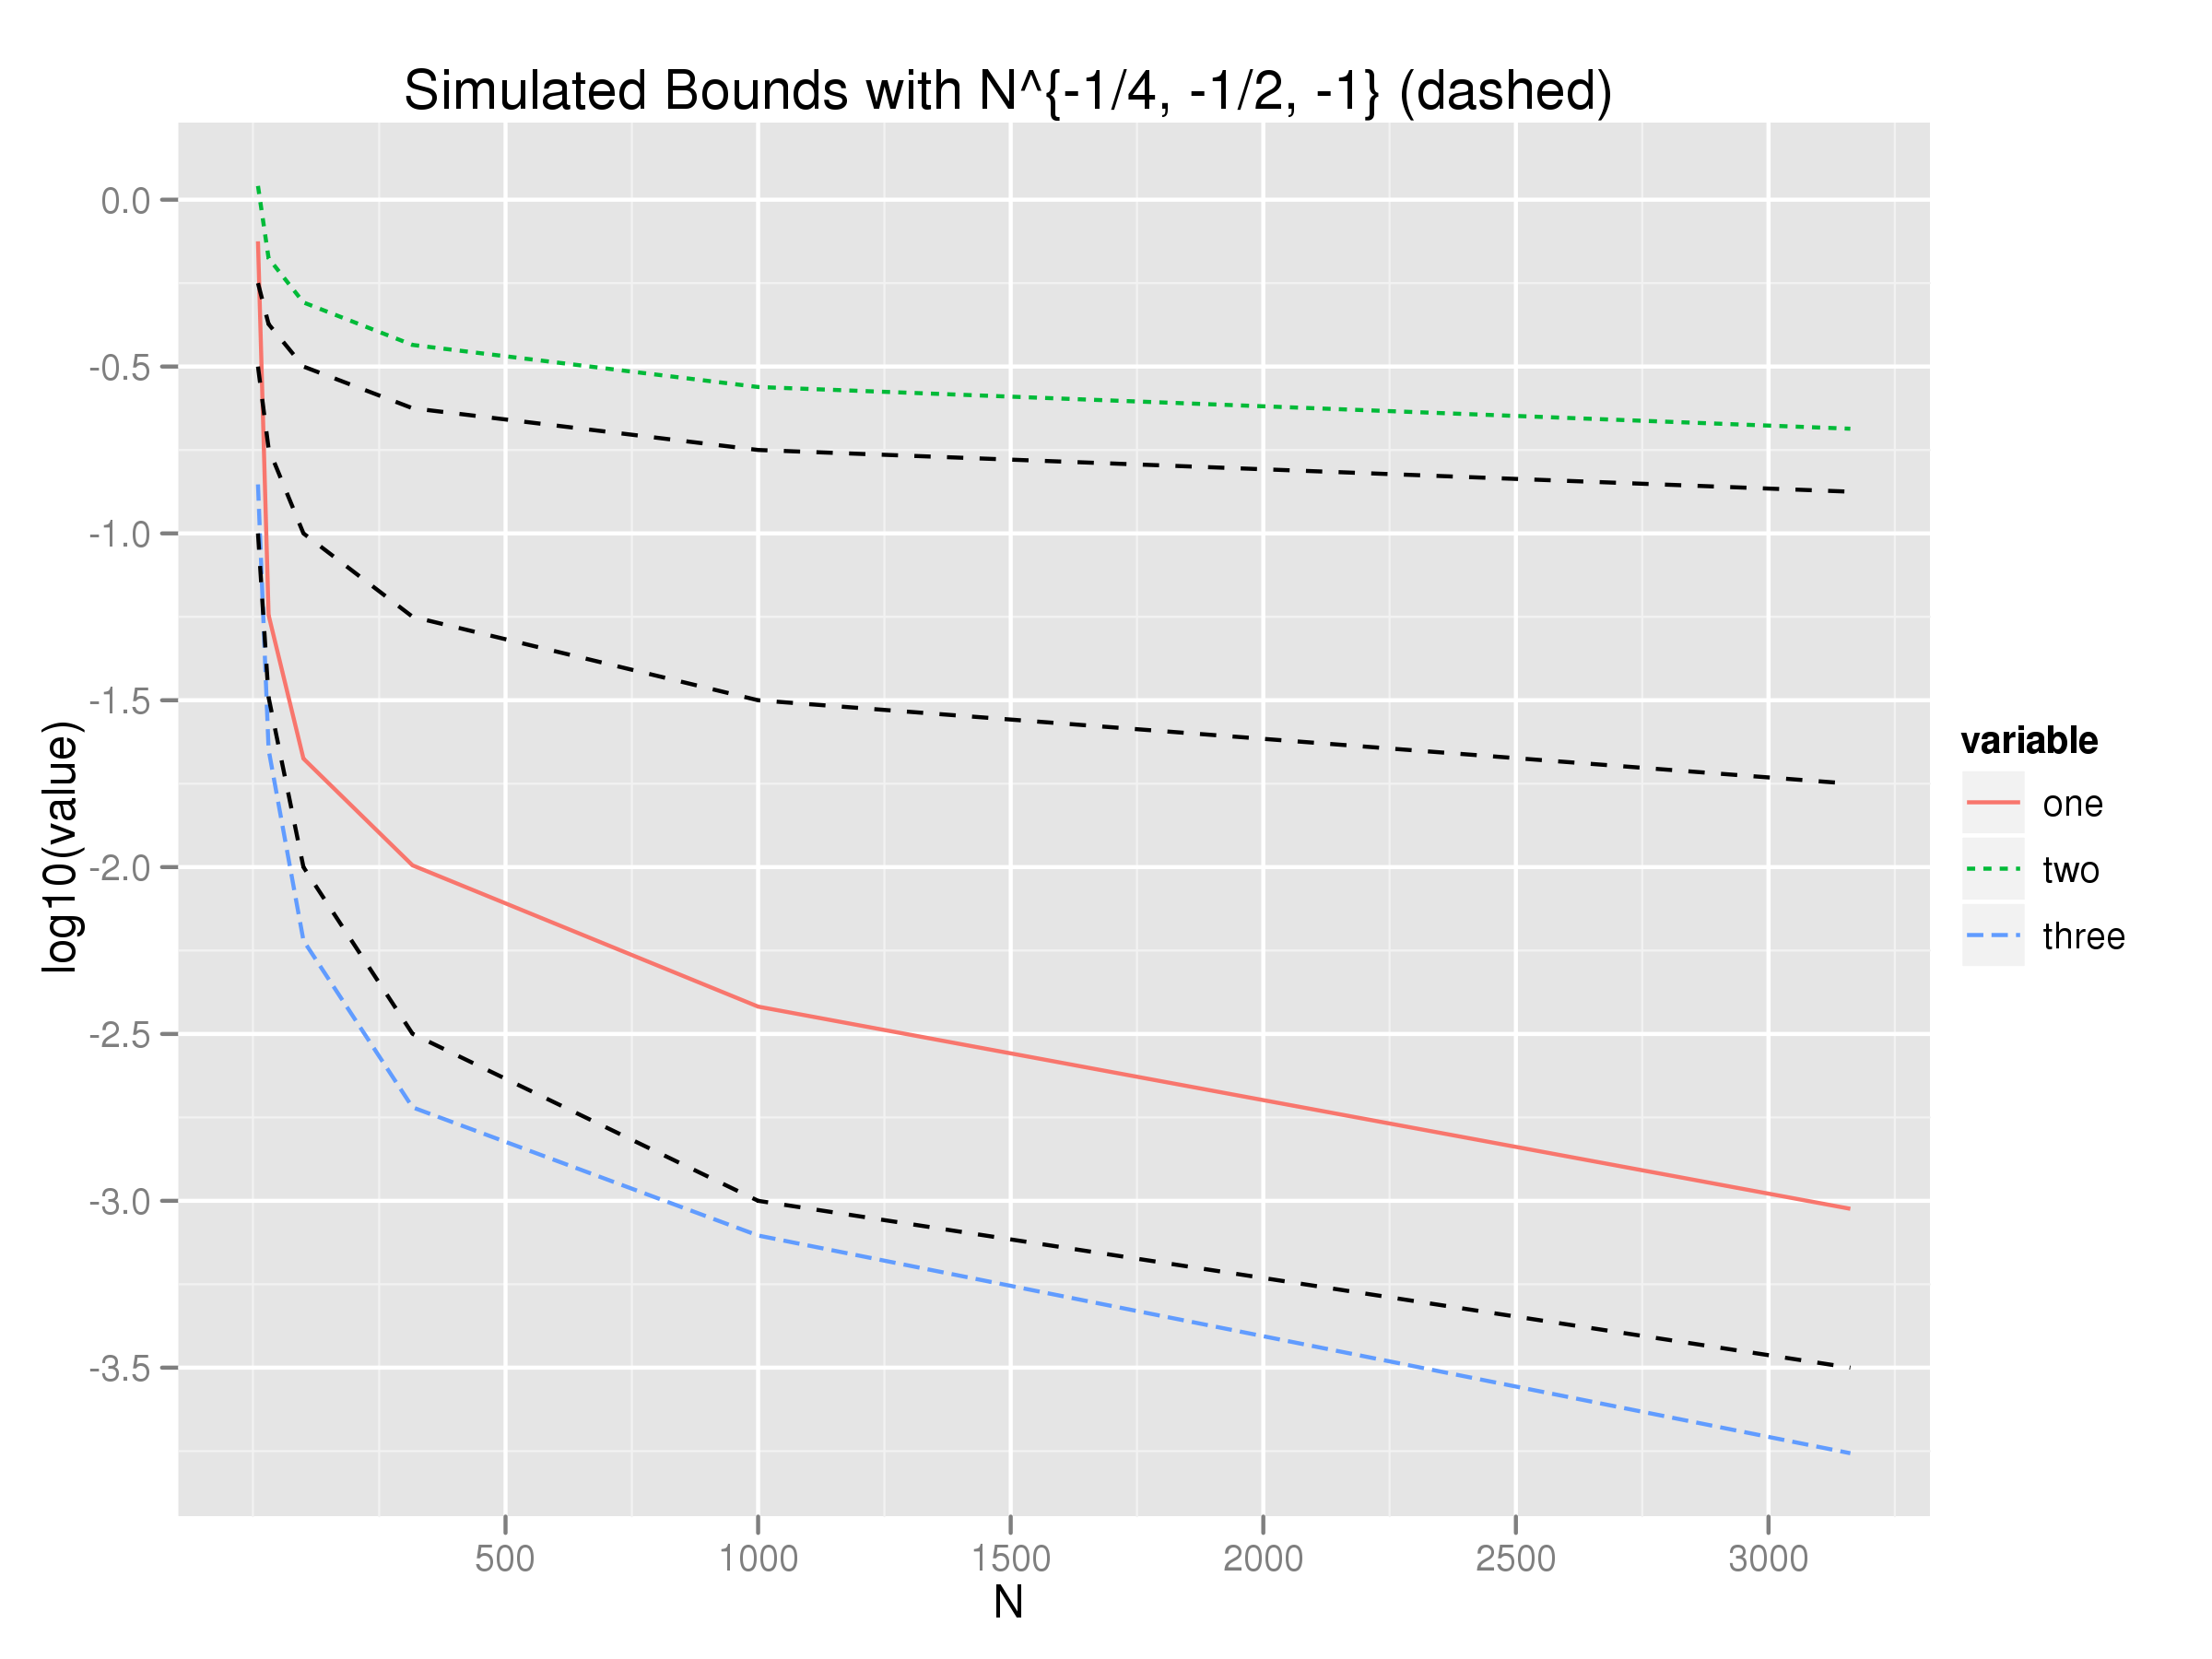
\includegraphics[scale=.5]{boundsexact.png}
 \end{figure}
\end{frame}

\begin{frame}{Twitter Example}
  \begin{figure}[!ht]
   \centering
   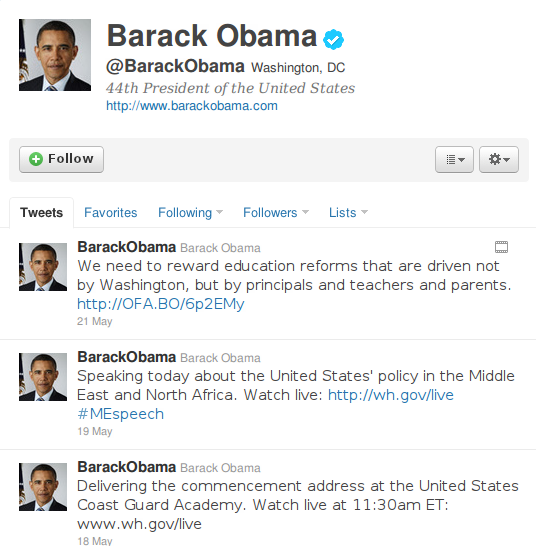
\includegraphics[scale=.3]{pres3.png}
   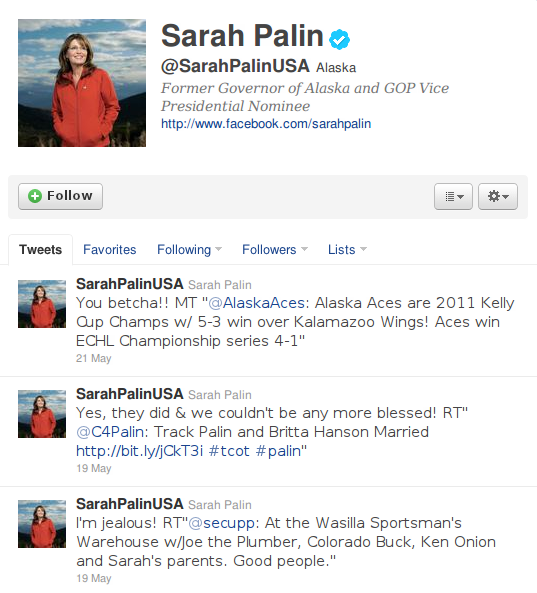
\includegraphics[scale=.3]{pres4.png}  
 \end{figure}
\end{frame}

\begin{frame}[fragile]{Twitter Data}
  Raw: 
\begin{verbatim}
"BarackObama: We need to reward education reforms that are 
driven not by Washington, but by principals and teachers and
parents. http://OFA.BO/6p2EMy"
"SarahPalinUSA: You betcha!! MT \"@AlaskaAces: Alaska Aces 
are 2011 Kelly Cup Champs w/ 5-3 win over Kalamazoo Wings! 
Aces win  ECHL Championship series 4-1\""
\end{verbatim}
  After pre-processing:
\begin{verbatim}
"we need to reward education reforms that are driven not by 
washington but by principals and teachers and parents "
"you betcha mt alaskaaces alaska aces are  kelly cup champs 
w  win over kalamazoo wings aces win  echl championship 
series "
\end{verbatim}
\end{frame}

\begin{frame}{Twitter Example}
  $p < .001$:
    \begin{figure}[!ht]
   \centering
   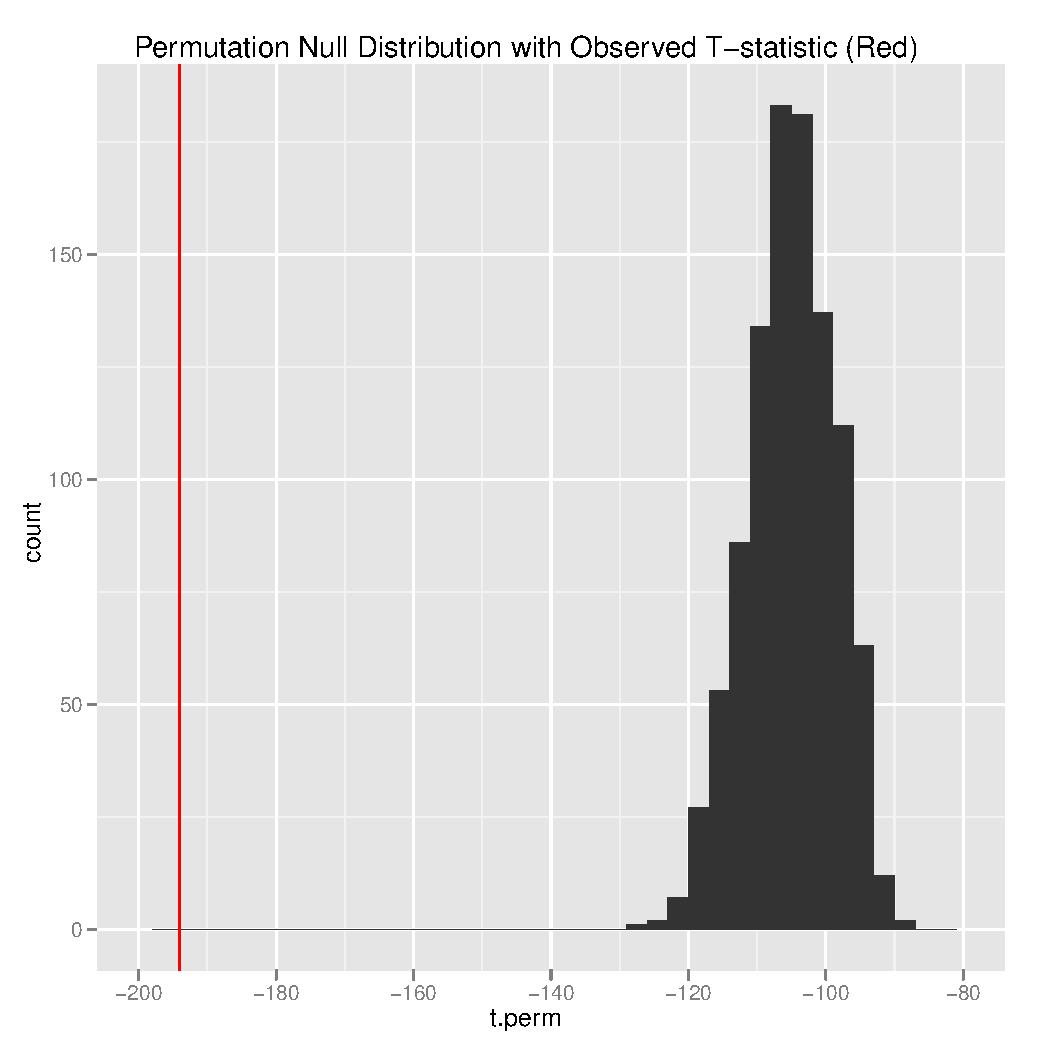
\includegraphics[scale=.4]{pres6.pdf}  
 \end{figure}
\end{frame}

\begin{frame}{Power Simulations at .05 Level}
   \begin{figure}[!ht]
   \centering
   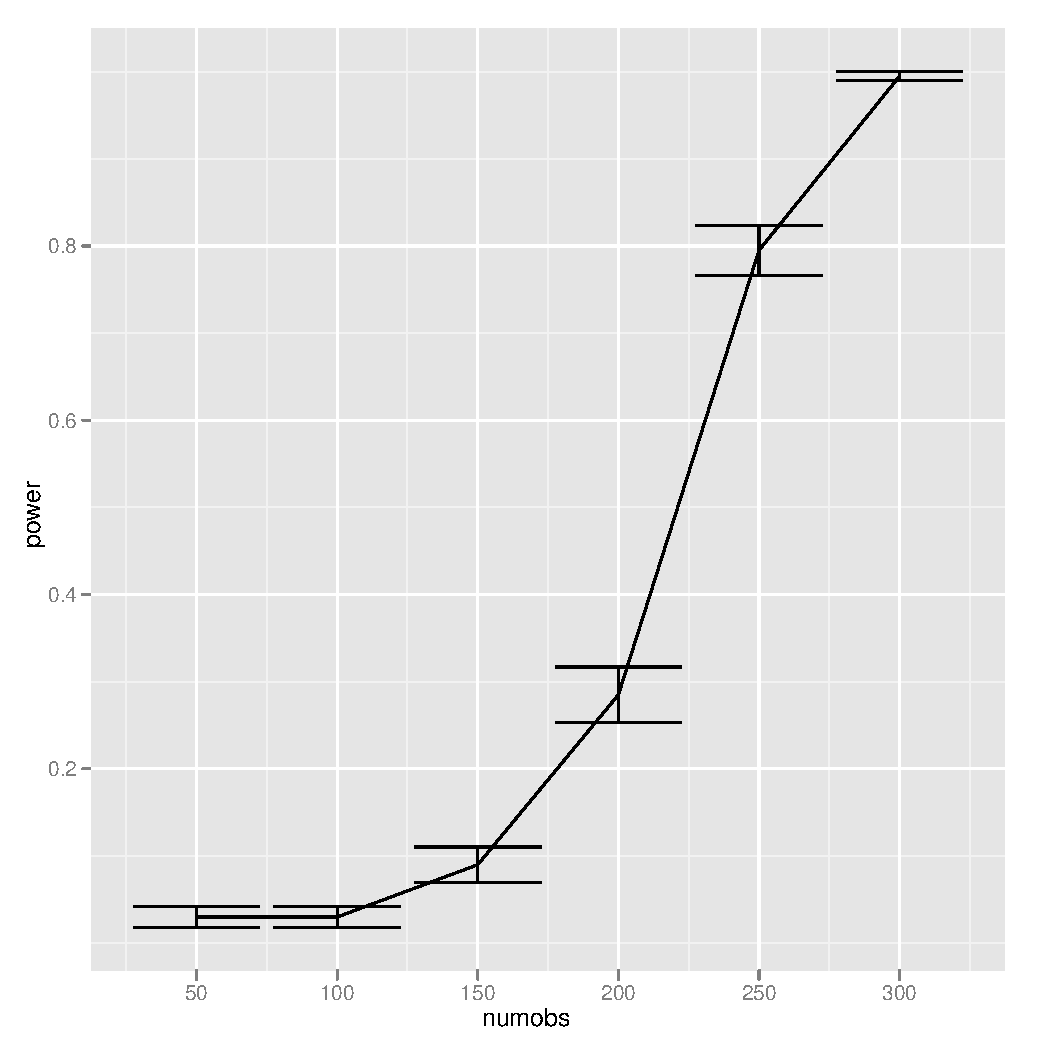
\includegraphics[scale=.4]{pres7.pdf}  
 \end{figure}
\end{frame}

\begin{frame}{Future Work}
  \begin{itemize}
  \item Generalize theory for higher dimensional settings and/or
    non-linear regression methods \pause
  \item Develop similarities with Hotelling's $T^2$-test \pause
  \item Explore performance on different types of data, in particular,
    unstructured data such as images \pause
  \item Heterogeneous data: optimal combinations of kernels
    via SDPs, KL divergence \pause
  \end{itemize}
\end{frame}

\begin{frame}[allowframebreaks]{References}
  \bibliographystyle{ieeetr}
  \bibliography{ncray}
\end{frame}

\end{document}
